\documentclass{article}
\usepackage{amsmath}
\usepackage{amssymb}
\usepackage{graphicx}
\usepackage{hyperref}
\usepackage[version=4]{mhchem}

\title{Problem 3}
\date{}

\begin{document}
\maketitle

\section*{Problem}
(AMC) In triangle \(A B C\), point \(F\) divides side \(A C\) in the ratio 1:2. Let \(E\) be the point of intersection of side \(B C\) and \(A G\) where G is the midpoint of \(B F\). Then point \(E\) divides side \(B C\) in the ratio\\
(A) \(1: 4\)\\
(B) \(1: 3\)\\
(C) \(2: 5\)\\
(D) \(4: 11\)\\
(E) \(3: 8\)\\
\centering
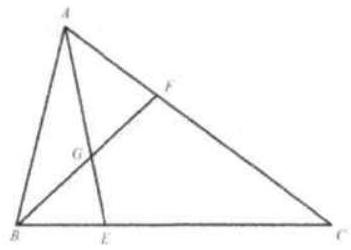
\includegraphics[width=\textwidth]{images/126.jpg}

\section*{Solution}
(B).\\
Method 1:\\
Draw \(F H\) parallel to line \(A G E\) (see figure). Then \(B E=E H\) because \(B G=G F\) and a line \((G E)\) parallel to the base \((H F)\) of a triangle \((H F B)\) divides the other two sides proportionally. By the same reasoning applied to triangle \(A E C\) with line \(F H\) parallel to base \(A E\), we see that \(H C=2 E H\), because \(F C=2 A F\) is given. Therefore \(E C=E H+H C=3 E H=3 B E\), and \(E\)\\
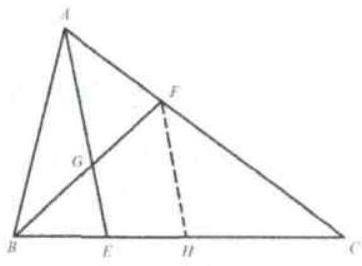
\includegraphics[width=\textwidth]{images/132.jpg} divides side \(B C\) in the ratio 1:3.

Method 2:\\
Applying Menelaus Theorem to \(\triangle A F G\) with the transversal points \(C, B\), and \(E\) :

\[
\begin{gathered}
\frac{A C}{F C} \cdot \frac{F B}{G B} \cdot \frac{G E}{A E}=1 \Rightarrow \frac{3}{2} \cdot \frac{2}{1} \cdot \frac{G E}{A E}=1 \Rightarrow \\
\frac{G E}{A E}=\frac{1}{3}
\end{gathered}
\]

Draw \(E D / / B F\) as shown in the figure. Let \(A F\) be \(2 n\) then \(F D\)\\
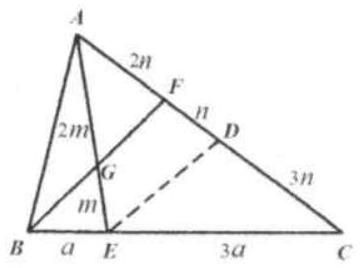
\includegraphics[width=\textwidth]{images/132(3).jpg} \(=n\) and \(D C=3 n . E\) divides side \(B C\) in the ratio \(1: 3\) as well.

\end{document}
